\chapter{Método Proposto}      \label{Metodo Proposto}

Otimizar os dispositivos nanofotônicos requer um trabalho de análise muito cuidadoso e assertivo. Cada simulação computacional pode demandar um tempo.

\section{Visão Geral}

Morbi a metus. Phasellus enim erat, vestibulum vel, aliquam a, posuere eu, velit. Nullam sapien sem, ornare ac, nonummy non, lobortis a, enim. Nunc tincidunt ante vitae massa. Duis ante orci, molestie vitae, vehicula venenatis, tincidunt ac, pede. Nulla accumsan, elit sit amet varius semper, nulla mauris mollis quam, tempor suscipit diam nulla vel leo. Etiam commodo dui eget wisi. Donec iaculis gravida nulla. Donec quis nibh at felis congue commodo. Etiam bibendum elit eget erat.


\section{Descrição do Problema}

Morbi a metus. Phasellus enim erat, vestibulum vel, aliquam a, posuere eu, velit. Nullam sapien sem, ornare ac, nonummy non, lobortis a, enim. Nunc tincidunt ante vitae massa. Duis ante orci, molestie vitae, vehicula venenatis, tincidunt ac, pede. Nulla accumsan, elit sit amet varius semper, nulla mauris mollis quam, tempor suscipit diam nulla vel leo. Etiam commodo dui eget wisi. Donec iaculis gravida nulla. Donec quis nibh at felis congue commodo. Etiam bibendum elit eget erat.


\section{Otimização por Aprendizado Profundo}

Maecenas ipsum velit, consectetuer eu, lobortis ut, dictum at, dui. In rutrum. Sed ac dolor sit amet purus malesuada congue. In laoreet, magna id viverra tincidunt, sem odio bibendum justo, vel imperdiet sapien wisi sed libero. Suspendisse sagittis ultrices augue. Mauris metus. Nunc dapibus tortor vel mi dapibus sollicitudin. Etiam posuere lacus quis dolor. Praesent id justo in neque elementum ultrices. Class aptent taciti sociosqu ad litora torquent per conubia nostra, per inceptos hymenaeos. In convallis. Fusce suscipit libero eget elit. Praesent vitae arcu tempor neque lacinia pretium. Morbi imperdiet, mauris ac auctor dictum, nisl ligula egestas nulla, et sollicitudin sem purus in lacus.

\begin{figure}[H]
    \centering
    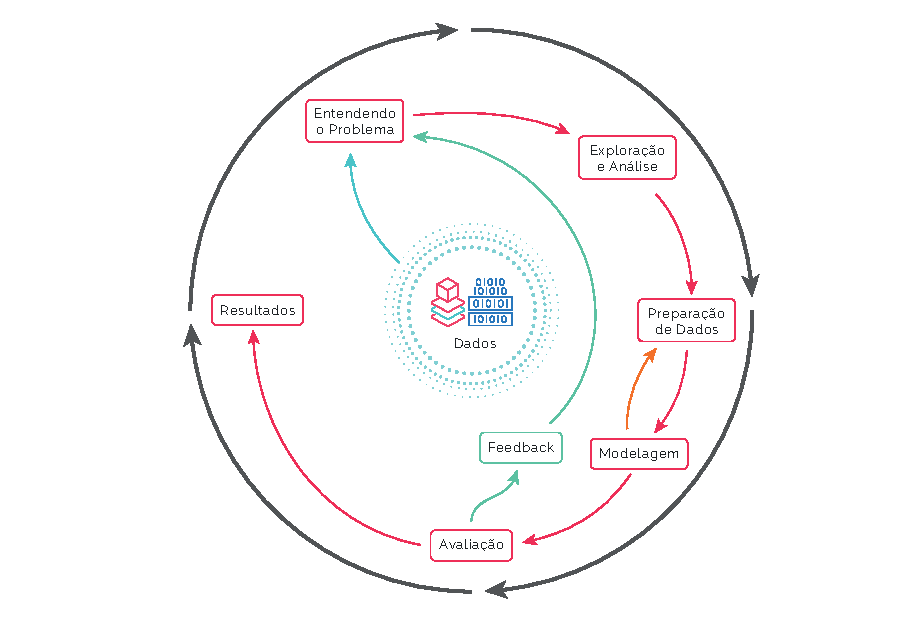
\includegraphics{04-Figuras/DataScienceDutyCicle.eps}
    \caption{Ciclo de trabalho de um projeto em ciência de dados.} \par
    Fonte: do Autor.
    \label{figura: DataScienceDutyCicle}
\end{figure}


\subsection{Construção do Banco de Dados}

O procedimento de otimização por inteligência artificial envolve, primeiramente, coletar os dados do problema e organizá-los em um banco de dados. Estes dados podem ser coletados por meio da API (\textit{Application Programming Interface}, ou ainda em português, Interface de Programação de Aplicativos) que o próprio COMSOL oferece. Uma API permite que aconteça troca de informações entre dois ou mais sistemas. Neste caso, a API \textit{COMSOL LiveLink for MATLAB} permite que o MATLAB possa controlar como as simulações numéricas do COMSOL acontecem, desde o processo de automatizá-las, à triagem desses dados para a construção do banco de dados.

Os dispositivos nanofotônicos são modelados e estudados a partir do software de simulação eletromagnética COMSOL. Nessa etapa, o próprio usuário constrói o dispositivo com as características geométricas e de operação que ele deve ter (como mostrado na Seção \ref{Modelando COMSOL} do Capítulo \ref{Revisao Bibliografica} deste documento).

Uma vez que esse estudo esteja estabelecido, o próximo passo é mapear variáveis que modificam a geometria do dispositivo simetricamente, respeitando assim a simetria do problema conforme estabelecido pela \textit{Teoria de Grupos} (ver Seção \ref{Embasamento Teorico} do Capítulo \ref{Revisao Bibliografica}). A Fig. mostra como esse processo de mapeamento é implementado. 

As mesmas variáveis que modificam simetricamente a geometria do dispositivo são usadas em um \textit{script} no MATLAB. A ideia por trás desse script é automatizar as simulações em loops de execução. A cada execução o matlab atribui valores randômicos para essas variáveis. Em termos práticos, isso significa que cada simulação de dispositivo terá uma geometria diferente para simular.


Ao final de uma simulação, os dados randômicos de geometria e a respectiva resposta em frequência são exportados em arquivos com a extensão \textit{.txt} e amarzenados em uma pasta no computadoor em um diretório definido também no mesmo script do MATLAB.

\begin{figure}[H]
    \centering
    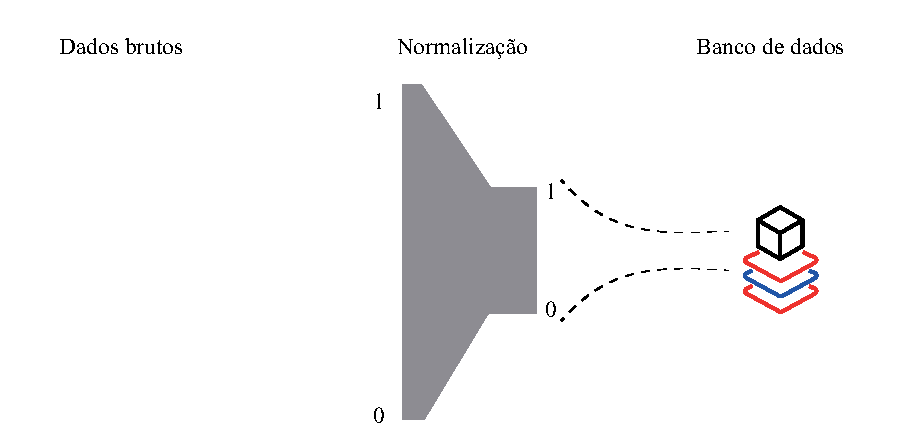
\includegraphics{04-Figuras/DatasetMounting.eps}
    \caption{Procedimento de contrução do dataset.} \par
    Fonte: do Autor.
    \label{figura: DatasetMounting}
\end{figure}

Foi desenvolvido também um outro script no MATLAB que é resposável por ler os dados gerados pelas simulações automatizadas. A função desse \textit{script} é ler todos os arquivos de simulação que foram gerados e montar o banco de dados em um único arquivo, onde os dados estão organizados de maneira sequencial (conforme o loop de simulação) e normalizados no intervalo $0\dotso 1$ (o procedimento de normalização está explicado na Seção deste Capítulo).

\begin{figure}[H]
    \centering
    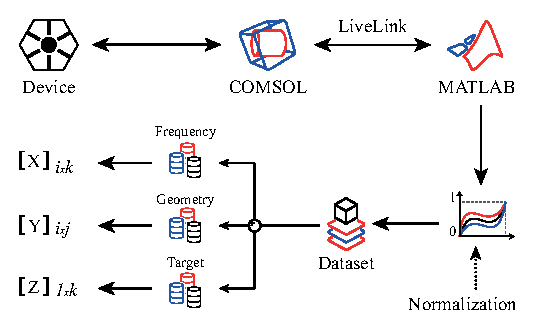
\includegraphics{04-Figuras/DatasetBuilding.eps}
    \caption{Procedimento de contrução do dataset.} \par
    Fonte: do Autor.
    \label{figura: DatasetBuilding}
\end{figure}

Assim, nessa etapa, são gerados três arquivos na extensão \textit{.csv}, cada qual entendidos como tensores, a saber:

\begin{itemize}
	\item \textbf{Resposta em Frequência} -- definido pelo tensor $[X]$, compreende as amplitudes discretizadas da resposta, sequenciadas linha-a-linha.
	\item \textbf{Geometria} -- definido pelo tensor $[Y]$, compreende os dados randômicos usados para modificar a geometria.
	\item \textbf{Espectro Desejado} -- definido pelo tensor $[Z]$, compreende à resposta em frequência desejada para o dispositivo definido pelo próprio projetista do dispositivo.
\end{itemize}









\begin{equation}
\label{eq:tensorY}
\mathbf{[Y]_{i,j}} =
\begin{bmatrix}
y_{1_{[1,1]}} & y_{2_{[1,2]}} & \cdots & y_{j_{[1,j]}}\\
y_{1_{[2,1]}} & y_{2_{[2,2]}} & \cdots & y_{j_{[2,j]}}\\
\vdots  & \vdots  & \ddots & \vdots\\
y_{1_{[i,1]}} & y_{2_{[i,2]}} & \cdots & y_{j_{[i,j]}}
\end{bmatrix},
\end{equation}

\noindent
where $j$ is the total number of the variables that modify the device's geometry and $i$ refers to the number of samples, i. e., the number of instances. The same reasoning applies to the construction of the frequency response dataset, whose are grouped into a tensor defined as:

\begin{equation}
\label{eq:tensorX}
\mathbf{[X]_{i,k}} =
\begin{bmatrix}
x_{1_{[1,1]}} & x_{2_{[1,2]}} & \cdots & x_{k_{[1,k]}}\\
x_{1_{[2,1]}} & x_{2_{[2,2]}} & \cdots & x_{k_{[1,k]}}\\
\vdots  & \vdots  & \ddots & \vdots\\
x_{1_{[i,1]}} & x_{2_{[i,2]}} & \cdots & x_{k_{[i,k]}}
\end{bmatrix}.
\end{equation}

Note that the instance number \textit{i} must be the same length for $\mathbf{[X]}$ and $\mathbf{[Y]}$, because geometry and frequency response need to be related. And, finally, the target frequency response is defined as a tensor:

\begin{equation}
\label{eq:tensorZ}
\mathbf{[Z]_{1,k}} =
\begin{bmatrix}
z_{1_{[1,1]}} & z_{2_{[1,2]}} & \cdots & z_{k_{[1,k]}}\\
\end{bmatrix}.
\end{equation}

As mentioned above, the tensor $\mathbf{[Z]}$ was made considering the ideal characteristics for the frequency response.


\subsection{Rede Neural Profunda}

A Rede Neural Profunda (sigla DNN, em inglês) foi desenvolvida na linguagem de programação Python com a \textit{framekork} Tensorflow. 

\subsection{Treinamento e Predição}

We train the DNN using Adam as an optimization algorithm, with a mean squared error (MSE) as a cost function. The training procedure is made by minimizing the cost function $C$, as shown in Eq. \ref{eq:costFunction}.

\begin{equation}
\label{eq:costFunction}
C = \frac{1}{n}\sum_{i=1}^{n}\left ( Y_{i} - \hat{Y}_{i} \right )^{2}.
\end{equation}


\subsection{Procedimento de Otimização}

Aenean placerat. In vulputate urna eu arcu. Aliquam erat volutpat. Suspendisse potenti. Morbi mattis felis at nunc. Duis viverra diam non justo. In nisl. Nullam sit amet magna in magna gravida vehicula. Mauris tincidunt sem sed arcu. Nunc posuere. Nullam lectus justo, vulputate eget, mollis sed, tempor sed, magna. Cum sociis natoque penatibus et magnis dis parturient montes, nascetur ridiculus mus. Etiam neque. Curabitur ligula sapien, pulvinar a, vestibulum quis, facilisis vel, sapien. Nullam eget nisl. Donec vitae arcu.

\begin{figure}[H]
    \centering
    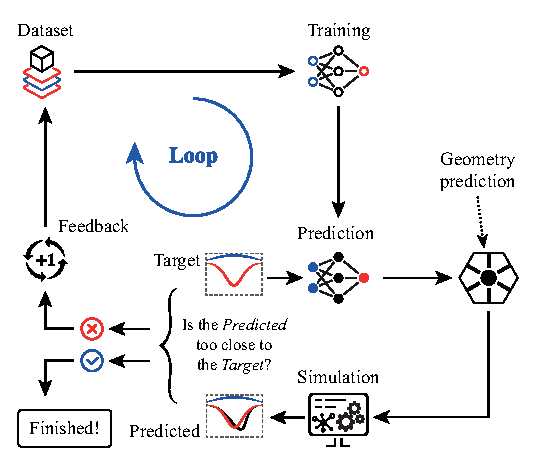
\includegraphics{04-Figuras/OptimizationAlgorithm.eps}
    \caption{Algorítmo de otimização.} \par
    Fonte: do Autor.
    \label{figura: OptimizationAlgorithm}
\end{figure}

Nam quis nulla. Integer malesuada. In in enim a arcu imperdiet malesuada. Sed vel lectus. Donec odio urna, tempus molestie, porttitor ut, iaculis quis, sem. Phasellus rhoncus. Aenean id metus id velit ullamcorper pulvinar. Vestibulum fermentum tortor id mi. Pellentesque ipsum. Nulla non arcu lacinia neque faucibus fringilla. Nulla non lectus sed nisl molestie malesuada. Proin in tellus sit amet nibh dignissim sagittis. Vivamus luctus egestas leo. Maecenas sollicitudin. Nullam rhoncus aliquam metus. Etiam egestas wisi a erat.


\section{Aplicação em Cristal Fotônico 2D}

Maecenas ipsum velit, consectetuer eu, lobortis ut, dictum at, dui. In rutrum. Sed ac dolor sit amet purus malesuada congue. In laoreet, magna id viverra tincidunt, sem odio bibendum justo, vel imperdiet sapien wisi sed libero. Suspendisse sagittis ultrices augue. Mauris metus. Nunc dapibus tortor vel mi dapibus sollicitudin. Etiam posuere lacus quis dolor. Praesent id justo in neque elementum ultrices. Class aptent taciti sociosqu ad litora torquent per conubia nostra, per inceptos hymenaeos. In convallis. Fusce suscipit libero eget elit. Praesent vitae arcu tempor neque lacinia pretium. Morbi imperdiet, mauris ac auctor dictum, nisl ligula egestas nulla, et sollicitudin sem purus in lacus.

\subsection{Princípio de Funcionamento}

Morbi a metus. Phasellus enim erat, vestibulum vel, aliquam a, posuere eu, velit. Nullam sapien sem, ornare ac, nonummy non, lobortis a, enim. Nunc tincidunt ante vitae massa. Duis ante orci, molestie vitae, vehicula venenatis, tincidunt ac, pede. Nulla accumsan, elit sit amet varius semper, nulla mauris mollis quam, tempor suscipit diam nulla vel leo. Etiam commodo dui eget wisi. Donec iaculis gravida nulla. Donec quis nibh at felis congue commodo. Etiam bibendum elit eget erat.

\begin{figure}[H]
    \centering
    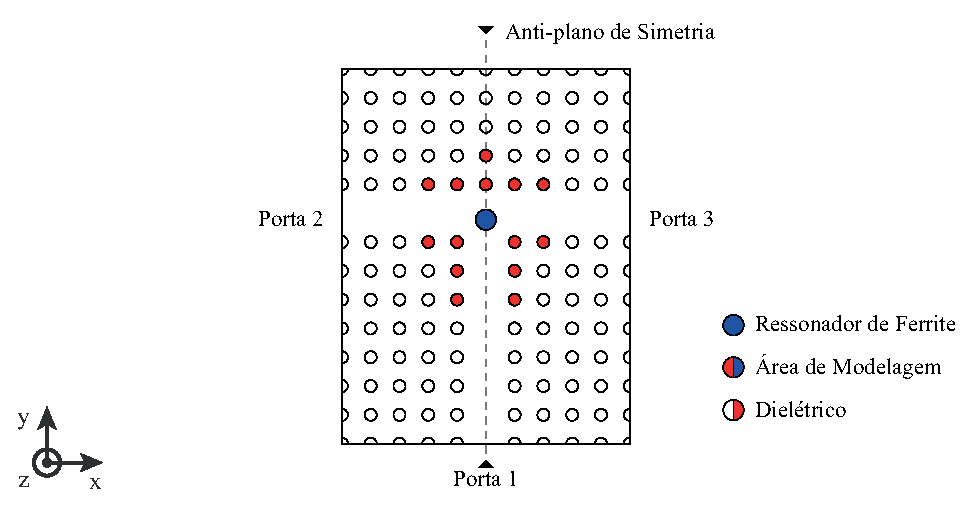
\includegraphics{04-Figuras/PhotonicCrystal.eps}
    \caption{Geometria do cristal fotônico.} \par
    Fonte: do Autor.
    \label{figura: PhotonicCrystal}
\end{figure}

\subsection{Ressonador Dipolo}

Nam quis nulla. Integer malesuada. In in enim a arcu imperdiet malesuada. Sed vel lectus. Donec odio urna, tempus molestie, porttitor ut, iaculis quis, sem. Phasellus rhoncus. Aenean id metus id velit ullamcorper pulvinar. Vestibulum fermentum tortor id mi. Pellentesque ipsum. Nulla non arcu lacinia neque faucibus fringilla. Nulla non lectus sed nisl molestie malesuada. Proin in tellus sit amet nibh dignissim sagittis. Vivamus luctus egestas leo. Maecenas sollicitudin. Nullam rhoncus aliquam metus. Etiam egestas wisi a erat.


\subsection{Ressonador Quadripolo}

Maecenas ipsum velit, consectetuer eu, lobortis ut, dictum at, dui. In rutrum. Sed ac dolor sit amet purus malesuada congue. In laoreet, magna id viverra tincidunt, sem odio bibendum justo, vel imperdiet sapien wisi sed libero. Suspendisse sagittis ultrices augue. Mauris metus. Nunc dapibus tortor vel mi dapibus sollicitudin. Etiam posuere lacus quis dolor. Praesent id justo in neque elementum ultrices. Class aptent taciti sociosqu ad litora torquent per conubia nostra, per inceptos hymenaeos. In convallis. Fusce suscipit libero eget elit. Praesent vitae arcu tempor neque lacinia pretium. Morbi imperdiet, mauris ac auctor dictum, nisl ligula egestas nulla, et sollicitudin sem purus in lacus.
